%%%%%%%%%%%%%%%%%%%%%%%%%%%%%%%%%%%%%%%%%
% Beamer Presentation
% LaTeX Template
% Version 2.0 (March 8, 2022)
%
% This template originates from:
% https://www.LaTeXTemplates.com
%
% Author:
% Vel (vel@latextemplates.com)
%
% License:
% CC BY-NC-SA 4.0 (https://creativecommons.org/licenses/by-nc-sa/4.0/)
%
%%%%%%%%%%%%%%%%%%%%%%%%%%%%%%%%%%%%%%%%%

%----------------------------------------------------------------------------------------
%	PACKAGES AND OTHER DOCUMENT CONFIGURATIONS
%----------------------------------------------------------------------------------------





\documentclass[
	10pt, % Set the default font size, options include: 8pt, 9pt, 10pt, 11pt, 12pt, 14pt, 17pt, 20pt
	%t, % Uncomment to vertically align all slide content to the top of the slide, rather than the default centered
	%aspectratio=169, % Uncomment to set the aspect ratio to a 16:9 ratio which matches the aspect ratio of 1080p and 4K screens and projectors
]{beamer}

\graphicspath{{figures/}{./}} % Specifies where to look for included images (trailing slash required)




\usepackage{booktabs} % Allows the use of \toprule, \midrule and \bottomrule for better rules in tables
\usepackage{multimedia}


\usepackage{hyperref}
\usepackage{outlines}
\usepackage{float}
\usepackage{caption}
\usepackage{subcaption}
\usepackage{makecell} 


% \usepackage{cases}
\usepackage{siunitx}
\usepackage{amssymb}
\usepackage{amsfonts}
\usepackage{mathtools}  % also loads amsmath
\renewcommand{\vec}[1]{\mathbf{#1}} % bold text instead of arrow


% \usepackage[backend=bibtex, 
%             style=phys, 
%             biblabel=brackets]{biblatex}



%----------------------------------------------------------------------------------------
%	THEME
%----------------------------------------------------------------------------------------

\usetheme{Madrid} %%%
\usefonttheme{default} % Typeset using the default sans serif font
% \usecolortheme{dolphin}
\definecolor{myblue}{RGB}{138,162,247}
\setbeamercolor{structure}{fg=myblue}
\setbeamercolor{section in head/foot}{bg=myblue}





% \usepackage{mathptmx} % Use the Times font for serif text
% \usepackage{palatino} % Use the Palatino font for serif text

%\usepackage{helvet} % Use the Helvetica font for sans serif text
% \usepackage[default]{opensans} % Use the Open Sans font for sans serif text
%\usepackage[default]{FiraSans} % Use the Fira Sans font for sans serif text
%\usepackage[default]{lato} % Use the Lato font for sans serif text

\useinnertheme{circles}
\useoutertheme{default}



% \setbeamertemplate{footline} % Uncomment this line to remove the footer line in all slides
% \setbeamertemplate{footline}[page number] % Uncomment this line to replace the footer line in all slides with a simple slide count
\setbeamertemplate{navigation symbols}{} % Uncomment this line to remove the navigation symbols from the bottom of all slides


% \usepackage{textpos} 
% \addtobeamertemplate{frametitle}{}{%
%     \begin{textblock*}{100mm}(0.96\textwidth,-0.85cm)
%         \includegraphics[height=0.8cm,width=0.8cm]{UiO_segl_pos-eps-converted-to.pdf}
%     \end{textblock*}}


%----------------------------------------------------------------------------------------
%	PRESENTATION INFORMATION
%----------------------------------------------------------------------------------------

\title[Predicting Graphene Kirigami Friction]{Predicting Frictional Properties of Graphene Kirigami Using Molecular Dynamics and Neural Networks}
\subtitle{Designs for a negative friction coefficient} 
\author[Mikkel Metzsch Jensen]{Mikkel Metzsch Jensen}
\institute[UiO]{University of Oslo}
\date[Juni 02, 2023]{Juni 02, 2023}

\titlegraphic{\flushleft\includegraphics[width=0.5\textwidth]{figures/MN_FYSISK_A_ENG.pdf}}

% \titlegraphic{\vspace{4cm}\flushright\includegraphics[width=2cm,height=2cm]{example-image-a}} 


\setbeamertemplate{bibliography item}{\insertbiblabel}
\usepackage[backend=bibtex, 
            style=phys, 
            biblabel=brackets]{biblatex}
\addbibresource{bibliography.bib}




%----------------------------------------------------------------------------------------
\begin{document}

%----------------------------------------------------------------------------------------
%	TITLE SLIDE
%----------------------------------------------------------------------------------------

\begin{frame}
	\titlepage % Output the title slide, automatically created using the text entered in the PRESENTATION INFORMATION block above
\end{frame}

%----------------------------------------------------------------------------------------
%	BODY
%----------------------------------------------------------------------------------------

\begin{frame}{Outline}
    \tableofcontents
\end{frame}
%
%%% New frame %%%
%
\section{Introduction} %%%%%%%%%%%%%%%%%%%%%%%%%%%%%%%%%%%%%%%%%%%%%%%%%%%%%%%%%%%%%
\subsection{Thesis overview}
\begin{frame}{Thesis overview}
	% \framesubtitle{Three main parts}
	\begin{enumerate}
		\setlength\itemsep{1em}
		\item \textbf{Sheet kirigami}: Alter a graphene sheet using atomic scale cuts and stretching
		\item \textbf{Forward simulation}: Calculate the frictional properties of the sheet using MD simulations
		\item \textbf{Accelerated search}: Use machine learning to replace the MD simulations and perform an accelerated search for new designs
	\end{enumerate}
	\vspace{2mm}
	
	Can we control the friction of a nanoscale Kirigami sheet through pattern design and straining of the sheet?

	\begin{alertblock}{}
        Can we control the friction of a nanoscale Kirigami sheet through pattern design and straining of the sheet?
    \end{alertblock}

	% \begin{itemize}
	% 	\item Can we utilize a coupling between load and stretch?
	% 	\item Negative friction coefficients
	% \end{itemize}
	
\end{frame}
%
%%% New frame %%%
%
\subsection{Motivation}
\begin{frame}{Motivation}
	\begin{itemize}
		\item Kirigami: Variation of origami with cuts permitted
		\item Desgins: Macroscale $\to$ nanoscale
	\end{itemize}
	\vspace*{10px}

	\begin{figure}
		\includegraphics[height=0.55\textheight]{figures/kirigami_example.jpg}
		\caption{Example of macroscale Kirigami designs implemented on a nanoscale using a focused ion beam (FIB). Black scale bars: \SI{1}{\mu m}. Reproduced from~\cite{Li_2018}.}
	\end{figure}	
\end{frame}
%
%%% New frame %%%
%
\begin{frame}{Motivation}
	\framesubtitle{Out-of-plane buckling}
	\vspace{0.5cm}
	
	\begin{itemize}
		\item Hanakata et al. \cite{Hanakata_2018,Hanakata_2020} found out-of-plane buckling with Kirigami designs
		\item Surface properties are predicted to be important for friction properties
		\begin{itemize}
			\item Asperity theory: Contact area
			\item Frenkel–Kontorova models: Commensurability
		\end{itemize}
	\end{itemize}
	% \vspace{1cm}

	\begin{figure}[H]
		\centering
		\begin{subfigure}[b]{0.49\textwidth}
			\centering
			\includegraphics[width=\textwidth]{../thesis/figures/theory/asperities_top.png}
			\caption{Small load.}
			\label{fig:asp_left}
		\end{subfigure}
		\hfill
		\begin{subfigure}[b]{0.49\textwidth}
			\centering
			\includegraphics[width=\textwidth]{../thesis/figures/theory/asperities_bottom.png}
			\caption{High load.}
			\label{fig:asp_right}
		\end{subfigure}
		\caption{Reproduced from~\cite{wiki:asperities}.}
	\end{figure}
\end{frame}
%
%%% New frame %%%
%
\begin{frame}{Motivation}
\framesubtitle{Contact area and commensurability}
\begin{figure}[H]
	\centering
	\begin{subfigure}[b]{0.46\textwidth}
		\centering
		\includegraphics[width=\textwidth]{figures/nano_asperity_contact.png}
		\caption{Numerical MD results using an amorphous carbon tip and a diamond sample. Reproduced from~\cite{mo_friction_2009} with permission from the Springer Nature.}
	\end{subfigure}
	\hfill
	\begin{subfigure}[b]{0.49\textwidth}
		\centering
		\includegraphics[width=\textwidth]{../thesis/figures/theory/graphene_rot.png}
		\caption{Experimental results of a graphene sheet sliding on graphite. Adapted from~\cite{DIENWIEBEL2005197}, reproduced from~\cite{Vanossi_2013} with permission from the American Physical Society.}
	\end{subfigure}
	% \caption{}
\end{figure}
\end{frame}
%
%%% New frame %%%
%
\subsection{System setup}
\begin{frame}{Outline}
    \tableofcontents[currentsection]
\end{frame}

\section{Creating a graphene Kirigami system} %%%%%%%%%%%%%%%%%%%%%%%%%%%%%%%%%%%%%%%%%%%%%%%%%%%%%%%%%%%%%
\begin{frame}{Creating a graphene Kirigami system}
\framesubtitle{System setup}
	\begin{figure}
		\centering    
		\movie[open,showcontrols=true,repeat]{\includegraphics[height=0.5\textwidth, keepaspectratio]{figures/sim_parts.png}}{figures/sim_parts.mov}
		\caption{Graphene sheet on a silicon substrate. Blue: Substrate, Red: Inner sheet, Grey: Pull blocks. }
	\end{figure} 
\end{frame}
%
%%% New frame %%%
%
\begin{frame}{Creating a graphene Kirigami system}
\framesubtitle{System setup}
	System size = ???

	\begin{figure}[H]
		\centering
		\begin{subfigure}[b]{0.5\textwidth}
			\centering
			\includegraphics[width=\textwidth]{../thesis/figures/system/system_sideview.png}
			\caption{Side view.}
		\end{subfigure}
		\begin{subfigure}[b]{0.5\textwidth}
			\centering
			\includegraphics[width=\textwidth]{../thesis/figures/system/system_topview_anno.png}
			\caption{Top view.}
		\end{subfigure}
		%    \caption{System configuration colorized to indicate NVE parts (red), thermostat parts (green) and rigid parts (blue). (a) Side view showing the sheet on top of the substrate. (b) Top view showing only the sheet.}
		%    \label{fig:system}
	\end{figure}
\end{frame}
%
%%% New frame %%%
%
\subsection{Kirigami}
\begin{frame}{Creating a graphene Kirigami system}
	\framesubtitle{Sheet Kirigami}

	Primitive lattice vectors
	\begin{align*}
		&\vec{a_1} = a \left(\frac{\sqrt{3}}{2}, -\frac{1}{2}\right)&  &\vec{a_2} = a \left(\frac{\sqrt{3}}{2}, \frac{1}{2}\right),& &|\vec{a_1}| = |\vec{a_2}| = a = \SI{2.46}{\text{Å}}.& 
	\end{align*}
	
	\begin{columns} 
		\begin{column}{.4\textwidth}
			Basis
			\begin{align*}
				\Big\{\Big(0,0\Big), \frac{a}{2}\Big(\frac{1}{\sqrt{3}}, 1 \Big) \Big\}.
			  \end{align*}
			Interatomic distance
			\begin{align*}
				\left|\left|\frac{a}{2}\Big(\frac{1}{\sqrt{3}}, 1 \Big)\right|\right| \approx \SI{1.42}{\text{Å}}.
			\end{align*}
		\end{column}
		\begin{column}{.6\textwidth}
			\begin{figure}[H]
				\centering
				\includegraphics[width=0.70\linewidth]{../thesis/figures/system/crystal.png}
				\caption{Graphene crystal structure.}
			\end{figure}
		\end{column}%
	\end{columns}
\end{frame}
%
%%% New frame %%%
%
\begin{frame}{Creating a graphene Kirigami system}
	\framesubtitle{Sheet Kirigami}
	\begin{figure}[H]
		\centering
		\includegraphics[width=0.7\linewidth]{../thesis/figures/system/atom_indexing.pdf}
		\caption{Graphene atom site indexing.}
	\end{figure}	
\end{frame}
%
%%% New frame %%%
%
\begin{frame}{Creating a graphene Kirigami system}
	\framesubtitle{Sheet Kirigami}
	\begin{figure}[H]
		\centering
		\includegraphics[width=0.7\linewidth]{../thesis/figures/system/center_indexing.pdf}
		\caption{Graphene center element indexing.}
	\end{figure}	
\end{frame}
%
%%% New frame %%%
%
\begin{frame}{Creating a graphene Kirigami system}
	\framesubtitle{Sheet Kirigami}
	\begin{figure}[H]
		\centering
		\begin{subfigure}[t]{0.48\textwidth}
			\centering
			\includegraphics[width=\textwidth]{../thesis/figures/system/pop_up_inspiration.png}
			\caption{Tetrahedron: Alternating perpendicular cuts producing a tetrahedron-shaped surface buckling when stretched. Reproduced from~\cite{new_pop_up}. }
		\end{subfigure}
		\hfill
		\begin{subfigure}[t]{0.48\textwidth}
			\centering
			\includegraphics[width=\textwidth]{../thesis/figures/system/honeycomb_inspiration.jpg}
			\caption{Honeycomb: Scotch\textsuperscript{TM} Cushion Lock\textsuperscript{TM}~\cite{cushion_wrap} producing a honeycomb-shaped surface buckling when stretched. Reproduced from~\cite{cushion_wrap}.}
		\end{subfigure}
		\hfill
		\caption{Macroscale kirigami cut patterns used as inspiration for the nanoscale implementation.}
	  \end{figure}
\end{frame}
%
%%% New frame %%%
%
\begin{frame}{Creating a graphene Kirigami system}
	\framesubtitle{Sheet Kirigami}
	

	\begin{figure}[H]
		\centering
		\begin{subfigure}[t]{0.49\textwidth}
			\centering
			\raggedleft
			\includegraphics[width=0.7\textwidth]{../thesis/figures/system/pop_up_inverse.pdf}
			% \caption{}
		  \end{subfigure}
		  \hfill
		  \begin{subfigure}[t]{0.49\textwidth}
			\centering
			\raggedright
			\includegraphics[width=0.7\textwidth]{../thesis/figures/system/pop_up_pattern.pdf}
			% \caption{}
		\end{subfigure}

	  \end{figure}
	  
	  
	  \begin{figure}[H]
		\centering
		\includegraphics[width=\linewidth]{../thesis/figures/system/pop_up_flavors.pdf}
	  \end{figure}
	  
\end{frame}
%
%%% New frame %%%
%
\begin{frame}{Creating a graphene Kirigami system}
	\framesubtitle{Sheet Kirigami}


	\begin{figure}[H]
		\centering
		\begin{subfigure}[t]{0.48\textwidth}
			\centering
			\raggedleft
			\includegraphics[width=0.7\textwidth]{../thesis/figures/system/honeycomb_inverse.pdf}
		  \end{subfigure}
		  \hfill
		  \begin{subfigure}[t]{0.48\textwidth}
			\centering
			\raggedright
			\includegraphics[width=0.7\textwidth]{../thesis/figures/system/honeycomb_pattern.pdf}
		\end{subfigure}
	  \end{figure}
	  
	  
	  \begin{figure}[H]
		\centering
		\includegraphics[width=\linewidth]{../thesis/figures/system/honeycomb_flavors.pdf}
	  \end{figure}
\end{frame}
%
%%% New frame %%%
%
\begin{frame}{Creating a graphene Kirigami system}
	\framesubtitle{Sheet Kirigami}
	Random walk 
	\begin{figure}[H]
		\centering
		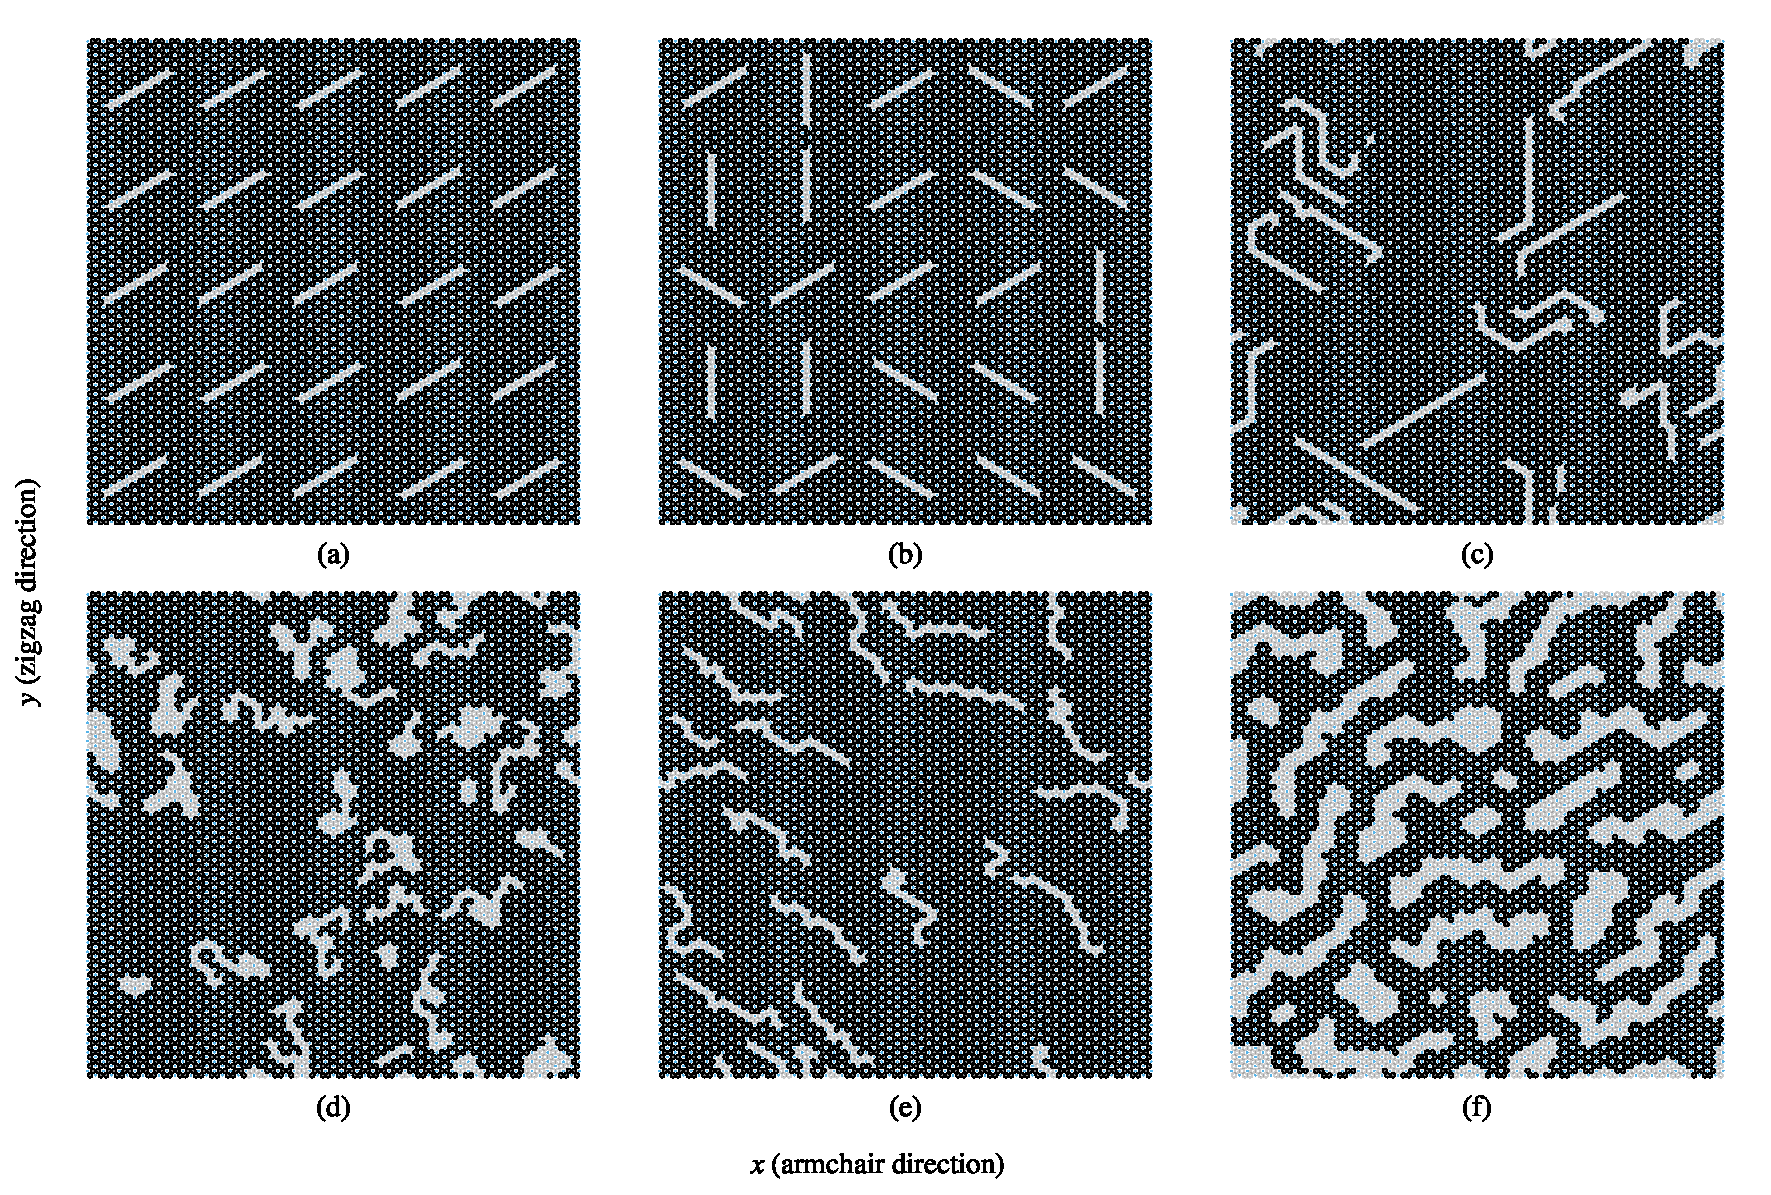
\includegraphics[width=0.8\linewidth]{../thesis/figures/system/RW_flavors.png}
	\end{figure}
\end{frame}
%
%%% New frame %%%
%
\begin{frame}{Creating a graphene Kirigami system}
	\framesubtitle{MD simulation}
	Integration. Newtons equation (NVE)
	\begin{align*}
		m_i \frac{d^2 \vec{r}_i}{dt^2} = \vec{F}_i = -\nabla U_i,
	\end{align*}
	Introducing the temperature (canonical ensemble: NVT) with the Langevin equation
	\begin{align*}
		m_i \frac{d^2 \vec{r}_i}{dt^2} &= \underbrace{-\nabla U_i}_{F_i} \ \underbrace{-\alpha \vec{v}_i}_{\text{Drag}}  + \underbrace{\vec{R}_i}_{\text{Fluctuation}}, \\
		\\
		\langle R \rangle &= 0, \qquad \langle R^2 \rangle = 2\alpha k_B T.
	\end{align*}

	% \begin{align*}
	% 	&\langle R \rangle = 0& &\langle R(t)^2 \rangle = 2\alpha k_BT&
	% \end{align*}
\end{frame}


\section{Pilot study} %%%%%%%%%%%%%%%%%%%%%%%%%%%%%%%%%%%%%%%%%%%%%%%%%%%%%%%%%%%%%
\begin{frame}{Outline}
    \tableofcontents[currentsection]
\end{frame}

\subsection{Friction metrics}
\begin{frame}{Pilot study}
	\framesubtitle{Friction metrics}

	\begin{itemize}
		\item Friction metrics?
		\item Stick slip?
	\end{itemize}
\end{frame}
%
%%% New frame %%%
%

\subsection{Out-of-plane buckling}
\begin{frame}{Pilot study}
	\framesubtitle{Out-of-plane buckling}
	\begin{figure}
		\centering    
		\movie[open,showcontrols=true]{\includegraphics[height=0.7\textheight, keepaspectratio]{figures/vacuum_stretch.png}}{figures/vacuum_stretch.mov}
		\caption{Kirigami sheet stretch in vacuum. Small tetrahedron pattern.}
	\end{figure} 

\end{frame}
%
%%% New frame %%%
%
\begin{frame}{Pilot study}
	\framesubtitle{Out-of-plane buckling}
	\begin{figure}
		\centering    
		\movie[open,showcontrols=true]{\includegraphics[height=0.7\textheight, keepaspectratio]{figures/contact_stretch.png}}{figures/contact_stretch.mov}
		\caption{Kirigami stretch in contact with Si-substrate.}
	\end{figure} 
\end{frame}
%
%%% New frame %%%
%
\begin{frame}{Pilot study}
	\framesubtitle{Out-of-plane buckling}
	\begin{figure}
		\includegraphics[height=0.7\textheight]{figures/contact_pct.pdf}
		\caption{Contact area approximation: Number of C-Si bonds within a threshold distance of 110\% the LJ interaction equilibrium distance.}
	\end{figure}	
\end{frame}


\subsection{Friction-strain profiles}
\begin{frame}{Pilot study}
	\framesubtitle{Friction-strain profiles}

	\begin{figure}[H]
		\centering
		\includegraphics[width=1\linewidth]{../thesis/figures/baseline/multi_stretch_area_compare.pdf}
	\end{figure}
\end{frame}
%
%%% New frame %%%
%
\begin{frame}{Pilot study}
	\framesubtitle{Friction-strain profiles}

	\begin{figure}[H]
		\centering
		\includegraphics[width=1\linewidth]{../thesis/figures/baseline/multi_stretch_mean_compare.pdf}
	\end{figure}
\end{frame}
%
%%% New frame %%%
%
\subsection{Negative friction coefficient}
\begin{frame}{Pilot study}
	\framesubtitle{Negative friction coefficient}
	Load to sheet tension coupling 
	\begin{align*}
		F_t = TF_N, \qquad T = 6
	\end{align*}
	\begin{figure}[H]
		\centering
		\includegraphics[width=0.6\linewidth]{../thesis/figures/negative_coefficient/nanomachine.pdf}
		% \caption{Working sketch for a nanomachine design that aims to translate applied load (from the top of the figure) to a straining of the graphene sheet (shown in red). The black boxes connected to the graphene sheet represent the pull blocks in our system.}
		% \label{fig:nanomachine}
	\end{figure}	  
\end{frame}
%
%%% New frame %%%
%
\begin{frame}{Pilot study}
	\framesubtitle{Negative friction coefficient}

	\begin{figure}[H]
		\centering
		\includegraphics[width=\linewidth]{../thesis/figures/negative_coefficient/manual_coupling_tension_pop7_5_1.pdf}	
		\caption{Tetrahedron $(7,5,1)$}
	\end{figure}	
\end{frame}
%
%%% New frame %%%
%

\begin{frame}{Pilot study}
	\framesubtitle{Negative friction coefficient}

	\begin{figure}[H]
		\centering
		\includegraphics[width=\linewidth]{../thesis/figures/negative_coefficient/manual_coupling_tension_hon2215.pdf}	
	\caption{Honeycomb $(2,2,1,5)$}
	\end{figure}	
\end{frame}
%
%%% New frame %%%
%
\begin{frame}{Pilot study}
	\framesubtitle{Negative friction coefficient}
	\begin{figure}
		\centering    
		\movie[open,showcontrols=true]{\includegraphics[width=\textwidth, keepaspectratio]{figures/hon_stretch.png}}{figures/hon_stretch.mov}
		\caption{Honeycomb $(2,2,1,5)$ stretch.}
	\end{figure} 
\end{frame}
%
%%% New frame %%%
%
\section{Kirigami configuration search} %%%%%%%%%%%%%%%%%%%%%%%%%%%%%%%%%%%%%%%%%%%%%%%%%%%%%%%%%%%%%
\begin{frame}{Outline}
    \tableofcontents[currentsection]
\end{frame}
%
%%% New frame %%%
%
\begin{frame}{Kirigami configuration search}
	\framesubtitle{Dataset}
	% \footnotesize
	\begin{table}[H]
		\begin{center}
		\caption{Summary of the generated data points in the dataset.}
		\begin{tabular}{ | c | c | c | c | c |} \hline
		\textbf{Type} & \textbf{Configurations} & \textbf{Submitted} & \textbf{Final} & \textbf{Ruptures} \\ \hline
		Pilot study & 3 & 270 & 261 & \: 25 \: (9.58 \%)\\ \hline
		Tetrahedron & 68 & 3060 & 3015 & 391 (12.97 \%)\\ \hline
		Honeycomb & 45 & 2025 & 1983 & \: 80 \: (4.03 \%)\\ \hline
		Random walk & 100 & 4500 & 4401 & 622 (14.13 \%) \\ \Xhline{2\arrayrulewidth}
		Total & 214 (216) & 9855 & 9660 & 1118 (11.57 \%) \\ \hline
		\end{tabular}
		\end{center}
	\end{table}
\end{frame}
%
%%% New frame %%%
%
\begin{frame}{Kirigami configuration search}
	\framesubtitle{Dataset}
	\begin{figure}[H]
		\centering
		\includegraphics[width=0.9\linewidth]{../thesis/figures/ML/corrcoef_matrix.pdf}
		\caption{Pearson product-moment correlation coefficients. }
	  \end{figure}
\end{frame}
%
%%% New frame %%%
%
\begin{frame}{Kirigami configuration search}
	\framesubtitle{Dataset}
	Properties of interest
	\begin{align*}
		&\min F_{\text{fric}},& &\max F_{\text{fric}},& &\max \Delta F_{\text{fric}},& &\max \text{drop}.&
	\end{align*}
	\begin{figure}[H]
		\centering
		\includegraphics[width=0.7\linewidth]{../thesis/figures/stretch_profiles/PP_max_drop.pdf}
		\caption{Max drop property. Best candidates in the dataset.}
	  \end{figure}
\end{frame}
%
%%% New frame %%%
%
\subsection{Machine learning}
\begin{frame}{Kirigami configuration search}
	\framesubtitle{ML}

	\begin{itemize}
		\item Convolutional neural network
		\item Input: Configuration, strain and load
		\item Output: \underline{Mean friction}, maximum friction, contact area, porosity, \underline{rupture}, rupture strain
	\end{itemize}

	\begin{figure}[H]
		\centering
		\includegraphics[width=0.5\linewidth]{../thesis/figures/ML/VGGNet16.jpg}
		\caption{Illustration of the convolutional network architecture for the VGGNet-16 network. Reproduced from~\cite{VGGNet_16_image}.}
	  \end{figure}
\end{frame}
%
%%% New frame %%%
%
\begin{frame}{Kirigami configuration search}
	\framesubtitle{ML}

	\begin{table}[H]
		\begin{center}
		\footnotesize
		\caption{Evaluation of the final model performance.}
		\label{tab:final_model_eval}
		\begin{tabular}{ | c | c | c | c | c | c | c |} \hline
		  & \multicolumn{3}{c|}{$R^2$ [\num{e2}]} & Abs. [\num{e2}] & Rel. [\num{e2}]  & Acc. [\num{e2}] \\ \hline
		  & Mean $F_f$ & Max $F_f$ & Contact & Porosity & Rup.\ Strain & Rupture \\ \hline
		Validation  & 98.067 & 93.558 & 94.598 & 2.325 & 12.958 & 96.102 \\ \hline
		Tetrahedron & 88.662 & 85.836 & 64.683 & 1.207 & \phantom{0}5.880 & 99.762 \\ \hline
		Honeycomb   & 96.627 & 89.696 & 97.171 & 1.040 & \phantom{0}1.483 & 99.111 \\ \hline
		\end{tabular}
		\end{center}
	\end{table}
\end{frame}
%
%%% New frame %%%
%
\begin{frame}{Kirigami configuration search}
	\framesubtitle{ML}
	\begin{figure}[H]
		\centering
		\includegraphics[width=0.8\linewidth]{../figures/final_model_evaluation_slide.pdf}
		\caption{Visual evaluation of the final model predictions on the Tetrahedron $(7,5,1)$ and Honeycomb $(2,2,1,5)$ used in the pilot study.}
	\end{figure}  

\end{frame}
%
%%% New frame %%%
%
\subsection{Accelerated search}
\begin{frame}{Kirigami configuration search}
	\framesubtitle{Accelerated search}
	We generate an extended dataset. 
	\begin{itemize}
		\item Tetrahedron: \num{1.35e5} configurations 
		\item Honeycomb: \num{2.025e6} configurations
		\item Random walk: \num{e4} configurations
	\end{itemize}
\end{frame}
%
%%% New frame %%%
%
\begin{frame}{Kirigami configuration search}
	\framesubtitle{Accelerated search}
	\begin{figure}[H]
		\centering
		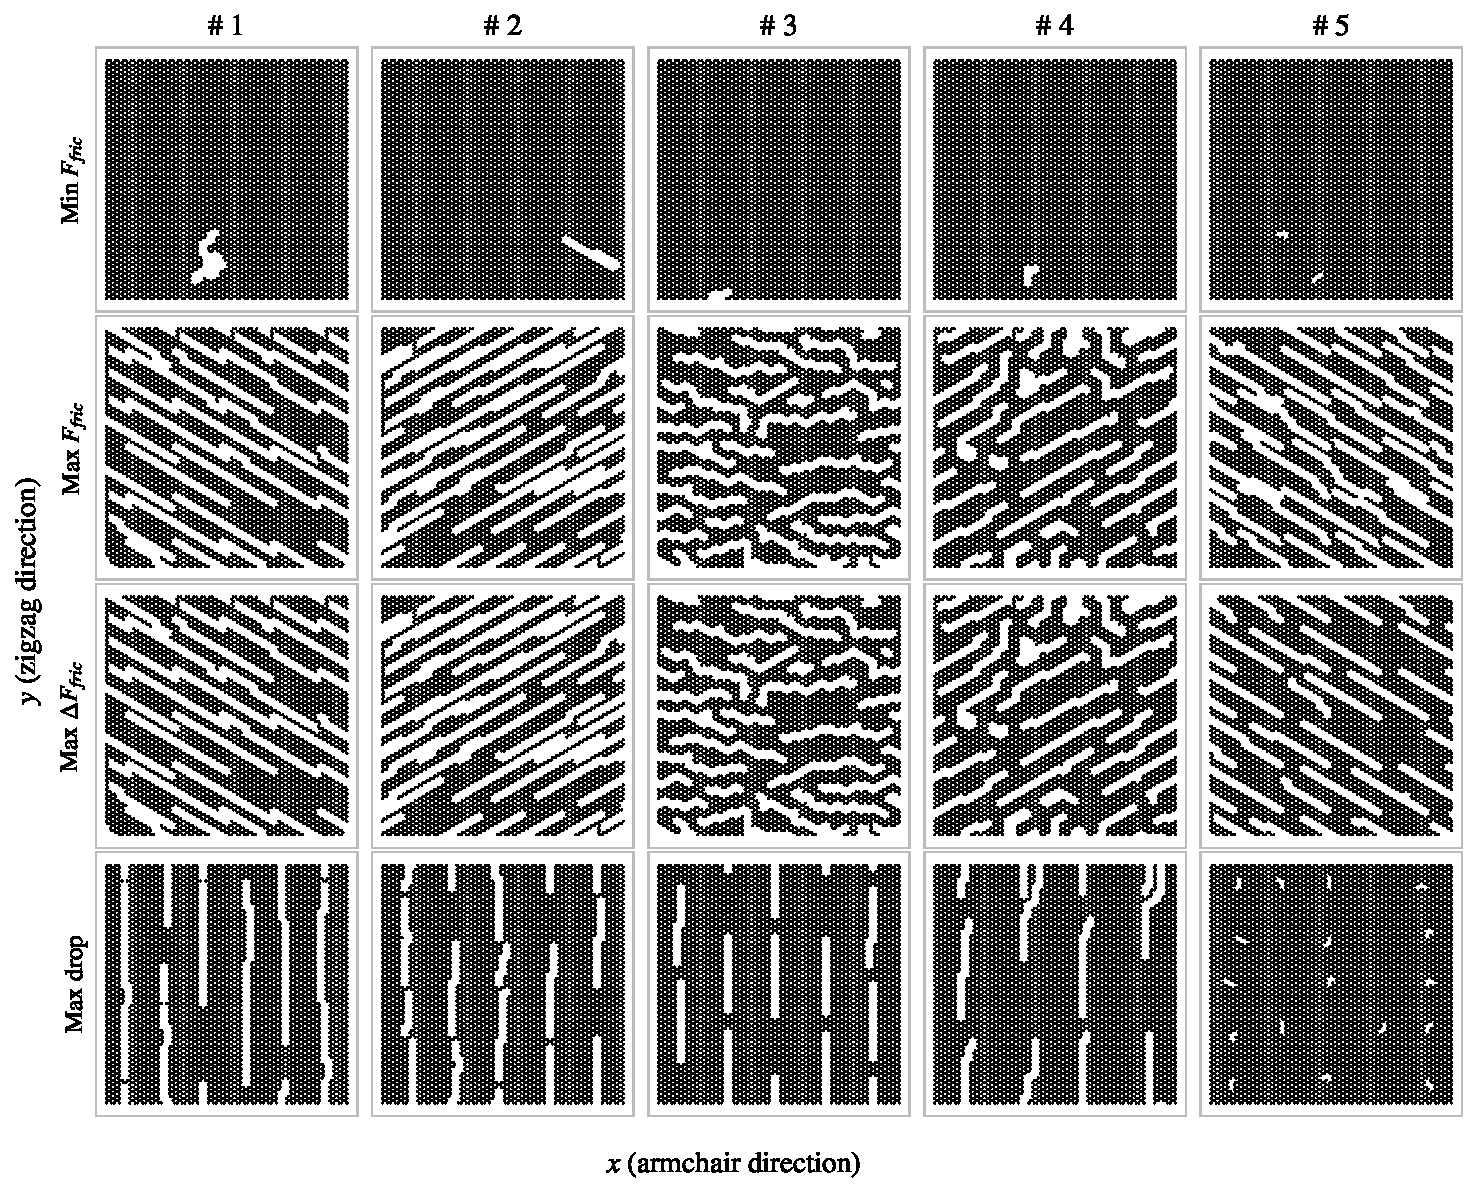
\includegraphics[width=0.8\linewidth]{../thesis/figures/search/RW_search_top5.png}
		\caption{Top 5 candidates for the accelerated search using the Random walk generator. }
	\end{figure}  
\end{frame}
%
%%% New frame %%%
%
\begin{frame}{Kirigami configuration search}
	\framesubtitle{Accelerated search}
	Translational variance
	\begin{figure}[H]
		\centering
		\begin{subfigure}[t]{0.49\textwidth}
			\centering
			\includegraphics[width=\textwidth]{../thesis/figures/search/ref_search_drop_pop_1_7_1_ref_search.pdf}
			\caption{Tetrahedron $(1,7,1)$ (60). Std = 0.08, Rel.\ Std = 1.13}
			\label{fig:tetra_171_trans}
		\end{subfigure}
		\hfill
		\begin{subfigure}[t]{0.49\textwidth}
			\centering
			\includegraphics[width=\textwidth]{../thesis/figures/search/ref_search_drop_pop_5_3_1_ref_search.pdf}
			\caption{Tetrahedron $(5,3,1)$ (60). Std = 0.13, Rel.\ Std = 1.61}
		\end{subfigure}
		\caption{Prediction of the max drop property for selected patterns using the machine learning model for all unique reference positions.}
	\end{figure}
\end{frame}
%
%%% New frame %%%
%
\begin{frame}{Kirigami configuration search}
	\framesubtitle{Accelerated search}
	Genetic algorithm based on Markov chain probability. 
	\begin{enumerate}
		\item Rank configurations by fitness score.
		\item Assign a mutation probability based on the ranking.
		\item Calculate target states from the best candidates.
		\item Mutate and repeat.
	\end{enumerate}
	Poor convergence on the mac drop property optimization
\end{frame}
%
%%% New frame %%%
%
\begin{frame}{Kirigami configuration search}
	\framesubtitle{Accelerated search}
	\begin{figure}[H]
		\centering
		\includegraphics[width=0.7\linewidth]{../thesis/figures/search/grad_cam_GA_RN_start_top0.pdf}
		\caption{Genetic algorithm suggestion from a mixed porosity start. Top: Friction-strain curve and configuration. Bottom: Grad-CAM analysis}
	\end{figure}  
\end{frame}
%
%%% New frame %%%
%
\begin{frame}{Kirigami configuration search}
	\framesubtitle{Accelerated search}
	Grad-CAM
	\begin{figure}[H]
		\centering
		\includegraphics[width=0.7\linewidth]{../thesis/figures/search/grad_cam_hon_3_3_5_3_12_0.pdf}
		\caption{Honeycomb $(3,3,5,3)$, ref = $(12,0)$.}
	\end{figure}  
\end{frame}
%
%%% New frame %%%
%




\section{Summary and outlook} %%%%%%%%%%%%%%%%%%%%%%%%%%%%%%%%%%%%%%%%%%%%%%%%%%%%%%%%%%%%%
\begin{frame}{Outline}
    \tableofcontents[currentsection]
\end{frame}


\begin{frame}{Summary and outlook}
	Key findings
	\begin{itemize}
		\item Non-monotonous relationship between friction and strain
		\item Coupled system can be exploited to achieve a negative friction coefficient
		\item Machine learning is feasible but more data is needed
	\end{itemize}
	Further studies:
	\begin{itemize}
		\item Investigation of the underlying mechanism
		\begin{itemize}
			\item Commensurability hypothesis can be investigated by varying scan angle
		\end{itemize}
		\item Friction-strain relationship at different physical conditions: temperature, sliding speed, spring stiffness. 
		\item Edge and thermostat effects.
		\item Improve dataset with active learning 
	\end{itemize}
\end{frame}






\begin{frame}[allowframebreaks]
	\frametitle{References}
	\printbibliography
	% \bibliographystyle{apalike}
	% \bibliographystyle{plain}
	% \printbibliography
	% \bibliography{./presentation/bibliography.bib}
\end{frame}



\end{document} 


